
\documentclass[11pt]{article}

\usepackage{common}
\usepackage{hyperref}
\title{HW4: Latent Variables}
\author{Jonah Philion \\ jonahphilion@college.harvard.edu \\ \href{https://github.com/jonahthelion/cs287-s18/tree/master/HW2}{github}}
\begin{document}

\maketitle{}
\section{Introduction}

In this problem set, we attempt to generate reasonable looking MNIST images using two models. With the VAE we model $p(X|z)=\text{Bin}(X|f(z))$ and $p(z|X) = N(z|\mu(X),\Sigma(X))$. The functions $\mu,\Sigma,f$ are parameterized as MLPs. The GAN trains a generator $G$ to generate images into a distribution which is indistinguishable from the distribution of the data $D$.

\section{VAE}
Data during training is a collection of handwritten digits $X=\{x_i\}$, where $x_i \in \{0,1\}^{24 \times 24}$. The encoder predicts a $\mu \in \mathbb{R}^2$ and $\Sigma \in \mathbb{R}^2$ for every input. We use the re-parameterization trick from the original VAE paper to allow gradients to flow through decoder to encoder.\\
The encoder used is an MLP with ReLU activation $24 \times 24 \rightarrow 50 \rightarrow 50 \rightarrow 4$ where the first two outputs are interpreted as $\mu$ and the second two is the log of the diagonal of the covariance $\Sigma$. The decoder is an MLP with ReLU activation $2 \rightarrow 50 \rightarrow 50 \rightarrow 28 \times 28$.\\
Reconstruction loss is measured with average binary cross entropy between the output of the decoder and the input image $x_i$. The KL for the case $KL(p||q)$ where $q$ is spherical and $p$ is diagonal is
$$ KL = \frac{1}{2}(\Sigma.\texttt{sum()} + \mu.\texttt{pow(2).sum()}-2-\Sigma.\texttt{log().sum()}) $$
The reconstruction loss plus KL loss is equivalent to equation (10) in \href{https://arxiv.org/pdf/1312.6114.pdf}{Kingma}. The loss is averaged over the number of images in a batch. The sum of losses $XENT+ KL$ is minimized with \texttt{Adam} of 0.001 learning rate over the course of 40 epochs. Both losses are tracked over the course of training on the training set and validation set as shown in Figure \ref{fig:loss}.\\
Interpolation is shown in Figure \ref{fig:grid}. The embedded space is displayed in Figure \ref{fig:vaespace}. Examples of the decoder output on a grid of latent variables is shown in Figure \ref{fig:grid}.


 \begin{figure}
  \centering
  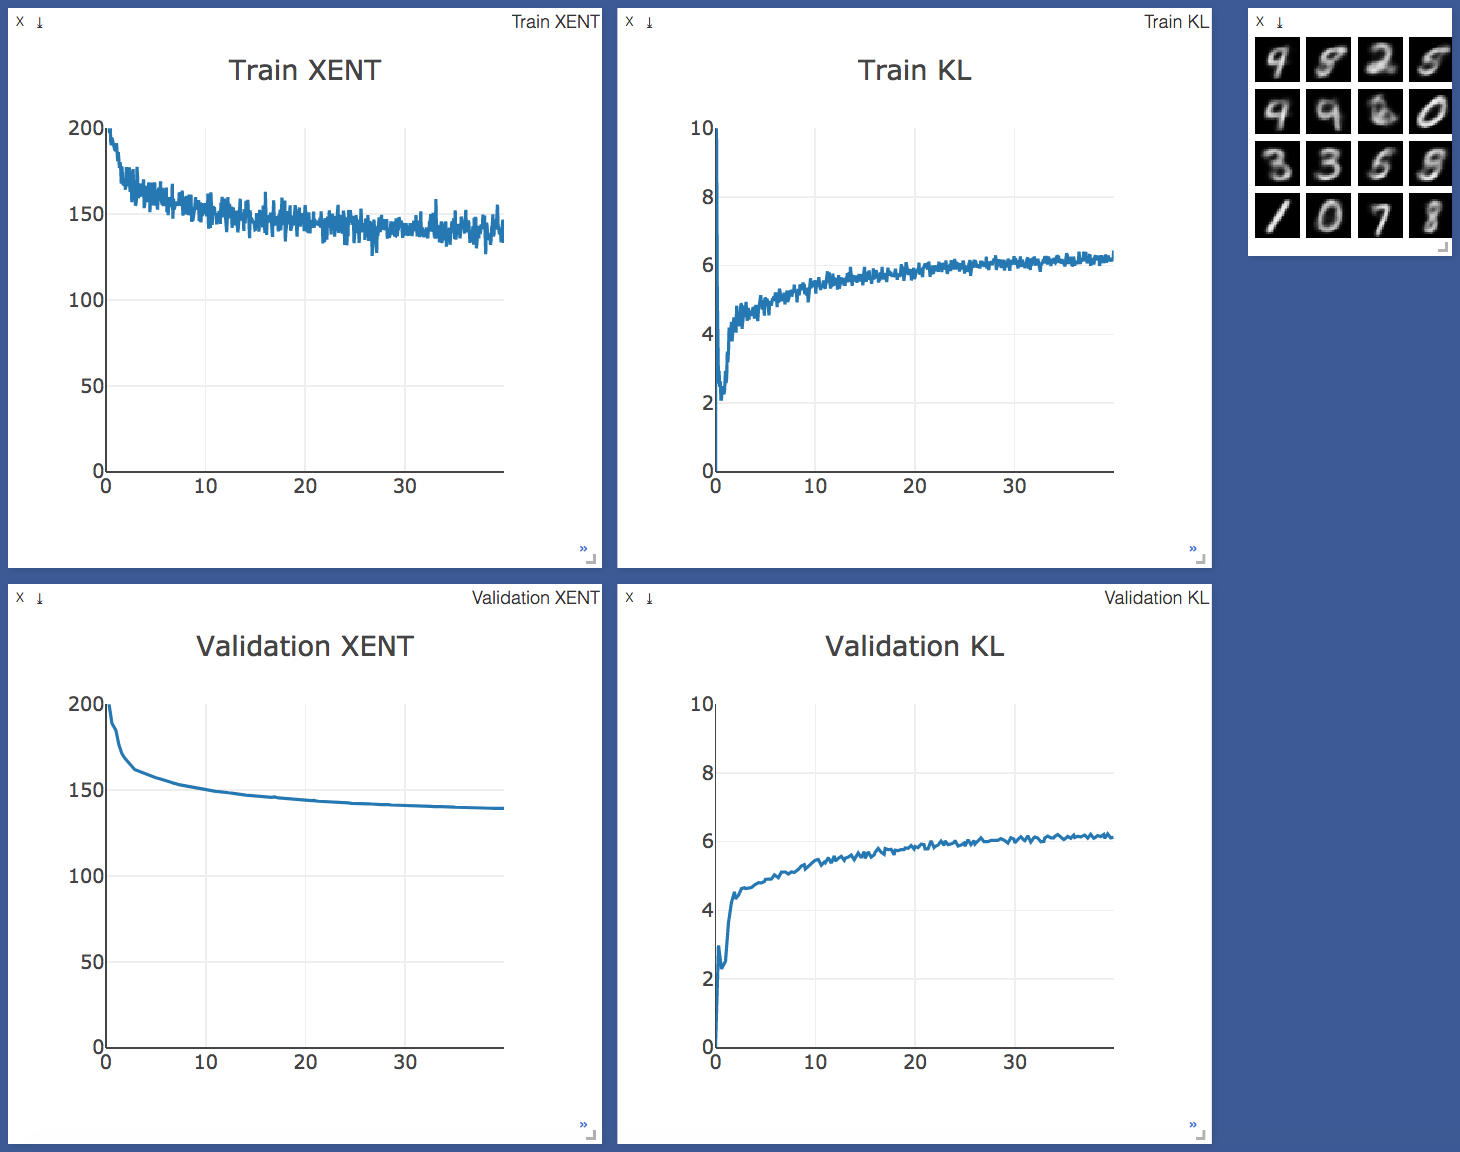
\includegraphics[width=9cm]{imgs/vae-train}
  \caption{\label{fig:loss} Visualization of training and validation loss for the VAE is handled by visdom. The x-axis is number of epochs through the training set in all cases. Example visualizations of the decoder's output in the top right are on random samples from $z$ which are sampled throughout training.}
\end{figure}

\begin{figure}
  \centering
  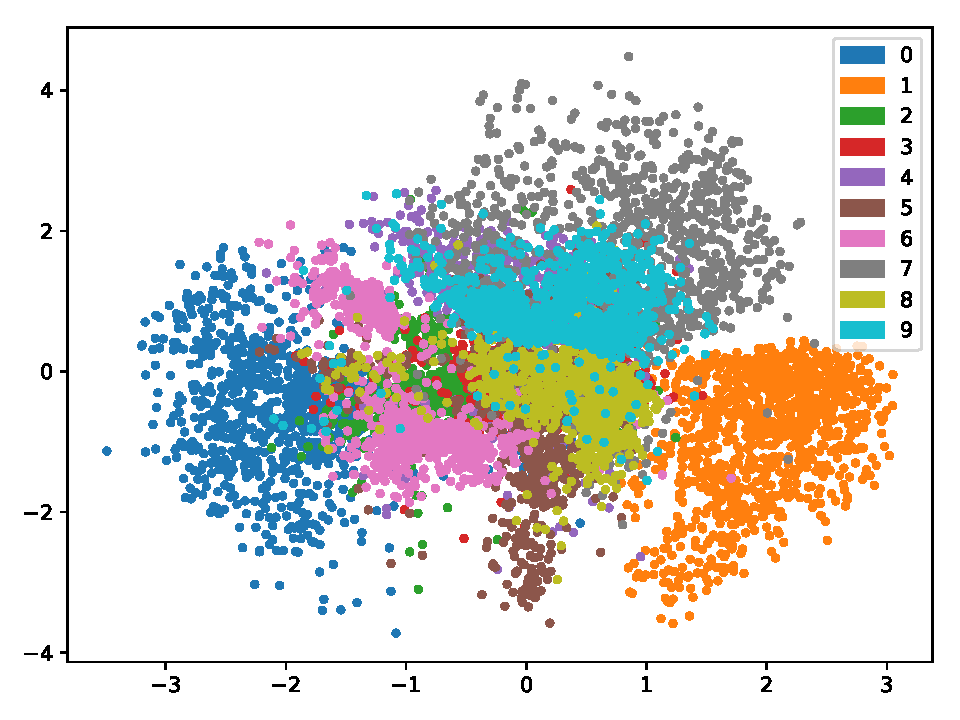
\includegraphics[width=9cm]{imgs/vae_mus2}
  \caption{The VAE model learns to separate the different digits without ever seeing a label. After training, on every test sample, we run the encoder and collect all the $\mu$ and ground truth labels. The $\mu$ are plotted and color coded by their ground truth label. The $\mu$ all together are roughly gaussian about the origin as enforced by the KL loss.}
  \label{fig:vaespace}
\end{figure}

\begin{figure}
  \centering
  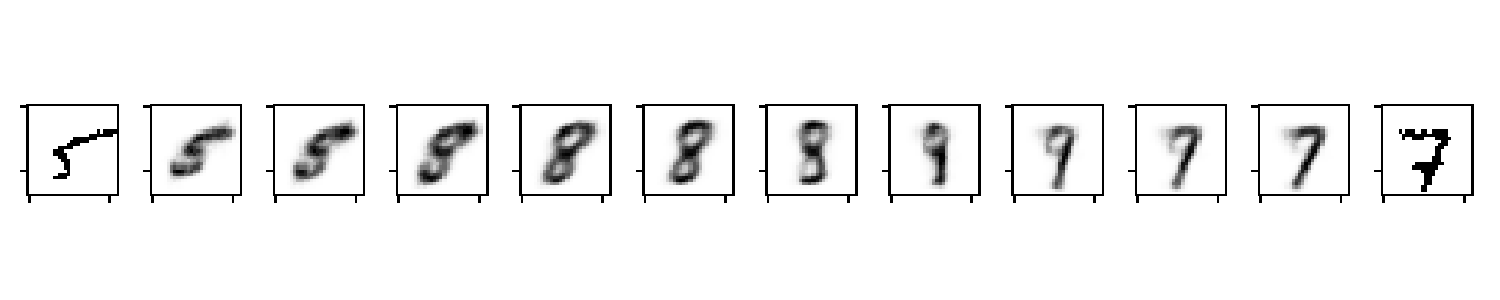
\includegraphics[width=15cm]{imgs/interp_vae2}
  \caption{\label{fig:grid} Two images from the test set are displayed on the far left and far right. We run the VAE encoder on both images, then decode 10 interpolations between the latent vectors. To smoothly move from an image of a 5 to an image of a 7, the model transitions to an 8 and then to a 9 and finally a 7. This trajectory is supported by Figure \ref{fig:vaespace}.}
\end{figure}

\begin{figure}
  \centering
  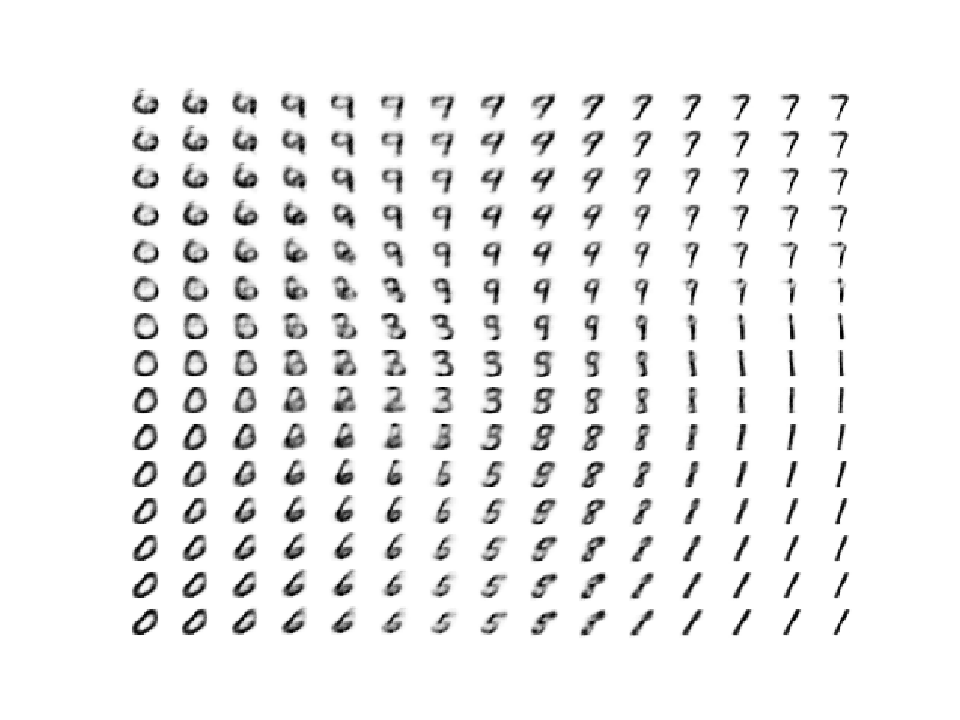
\includegraphics[width=15cm]{imgs/gridvae}
  \caption{\label{fig:grid} 15 latent vectors on a grid between -2 and 2 are decoded by the VAE into images. There is a sense in which the latent variable plotted on the $y$ axis encodes the angle of the digit.}
\end{figure}

\section{GAN}
To train our gan we consult Goodfellow's original \href{https://arxiv.org/pdf/1406.2661.pdf}{paper} and the Tutorial \href{https://github.com/soumith/ganhacks}{``How to train your GAN"}. Small latent dimensions are difficult to train so we use $h=150$.\\
The GAN decoder is identical to the decoder used in the VAE except ReLU is replaced with LeakyReLU and the final layer is \texttt{tanh} instead of linear. The discriminator has identical architecture to the encoder the VAE encoder except the discriminator has final dimension 1.\\
We train for 250 epochs with an Adam optimizer for both the discriminator and generator of learning rate .001. At each step, the 100  images in a batch are normalized to fall within $-1$ to $1$, we sample 100 latent vectors from a spherical gaussian of dimension $h$, and we decode these into images. The discriminator is then updated to differentiate between the data images and the decoded images. We next resample 100 latent vectors, apply the decoder, and update the generator to fool the discriminator into classifying the images as drawn from the data.\\
Noise Unif(0,.2) is added to every ground truth label. The discriminator loss and generator loss are tracked over the course of training and displayed in Figure \ref{fig:gantrain}. 36 random example decodings are displayed in Figure \ref{fig:gangrid}. A linear interpolation of two random latent vectors is shown in Figure \ref{fig:gan_12}.

\begin{figure}
  \centering
  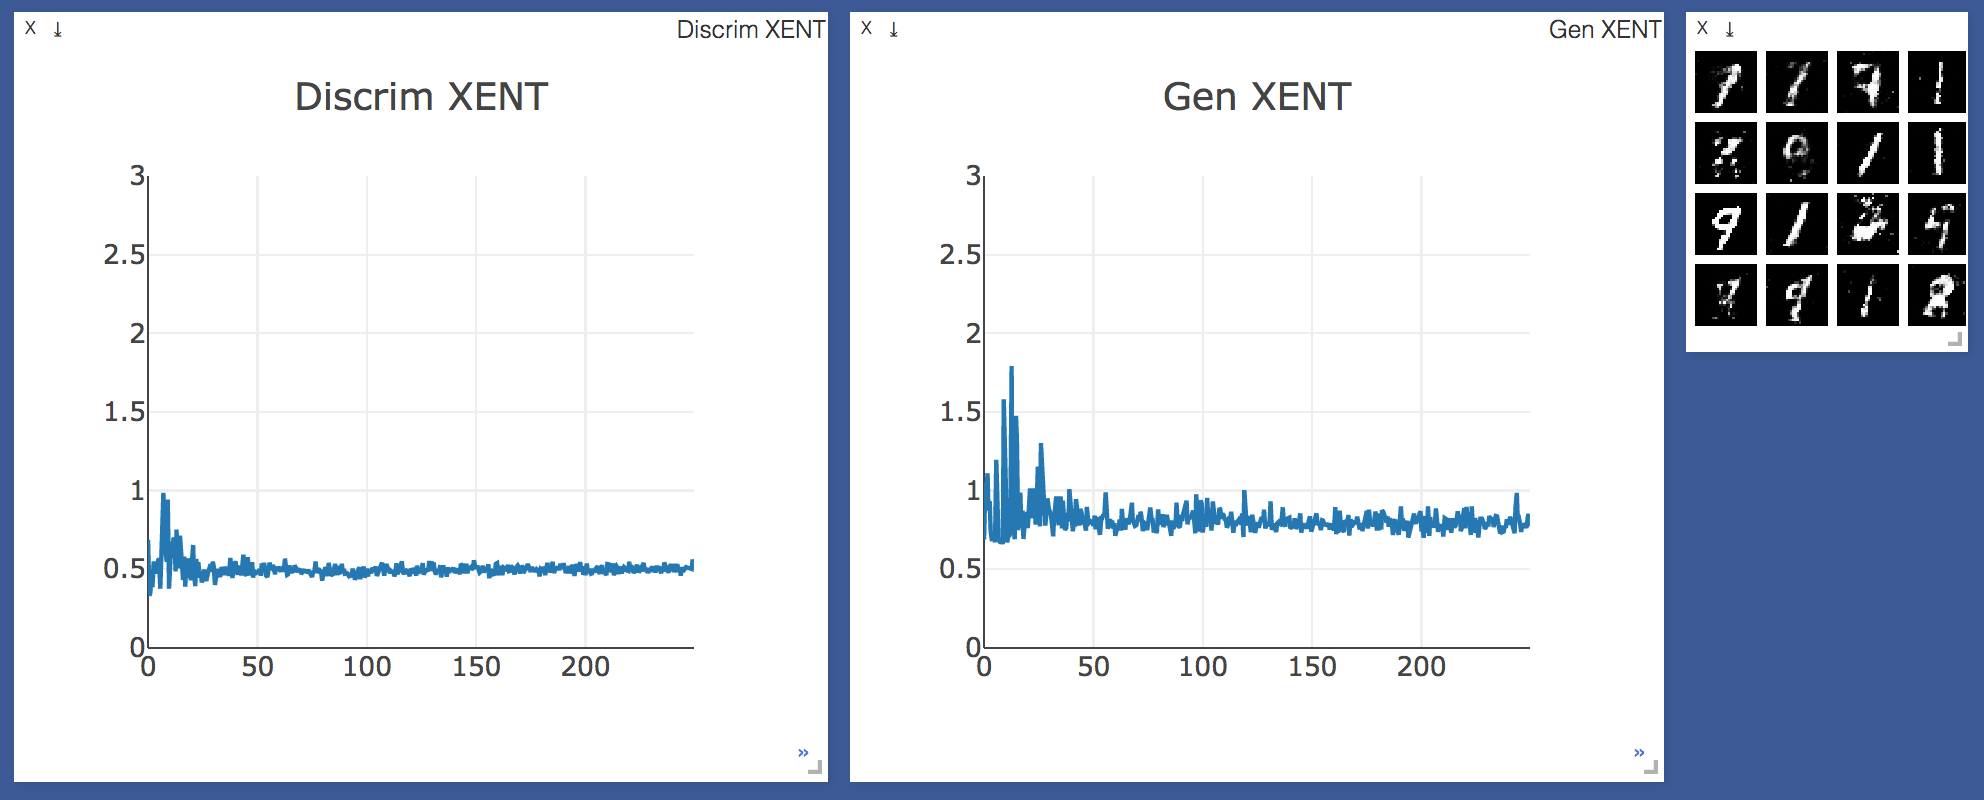
\includegraphics[width=15cm]{imgs/gan-train}
  \caption{\label{fig:gantrain} the leftmost image is the cross entropy of the discriminator on 100 data and 100 generated images during training of the GAN. The middle image is the cross entropy of the discriminator on 100 generated images where ground truth is defined as being drawn from the data. The rightmost images are example decoded images which are sampled every epoch.}
\end{figure}

\begin{figure}
  \centering
  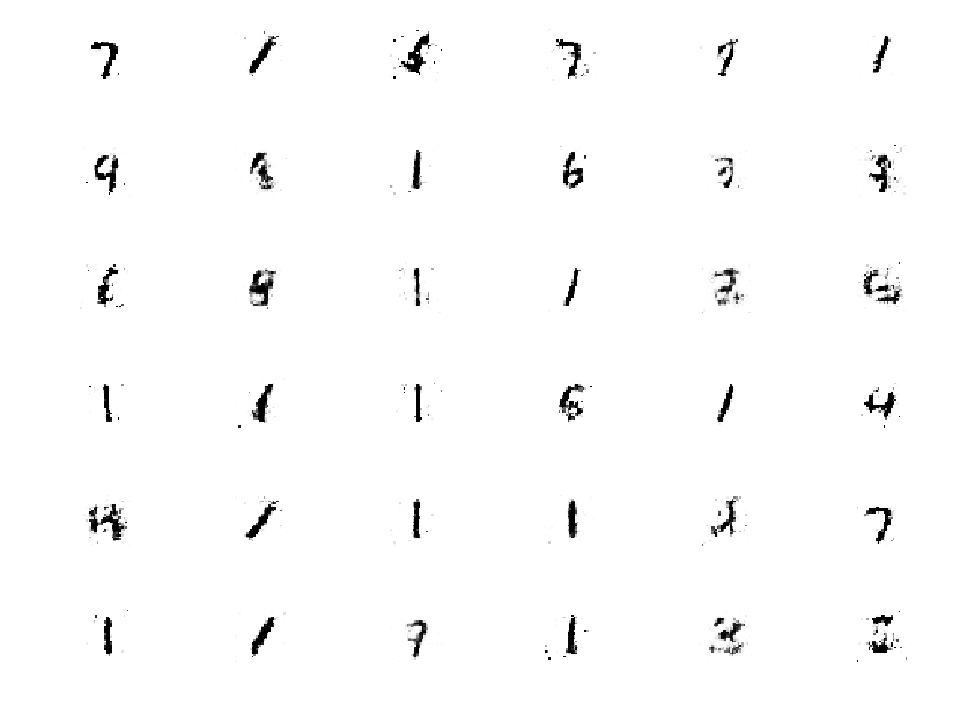
\includegraphics[width=15cm]{imgs/gan_decode2}
  \caption{\label{fig:gangrid} 36 latent vectors are randomly sampled from the GAN space and the output of the GAN decoder on these vectors is plotted in no particular order. The images aren't as smooth as the VAE images but they are also less fuzzy which is a plus.}
\end{figure}

\begin{figure}
  \centering
  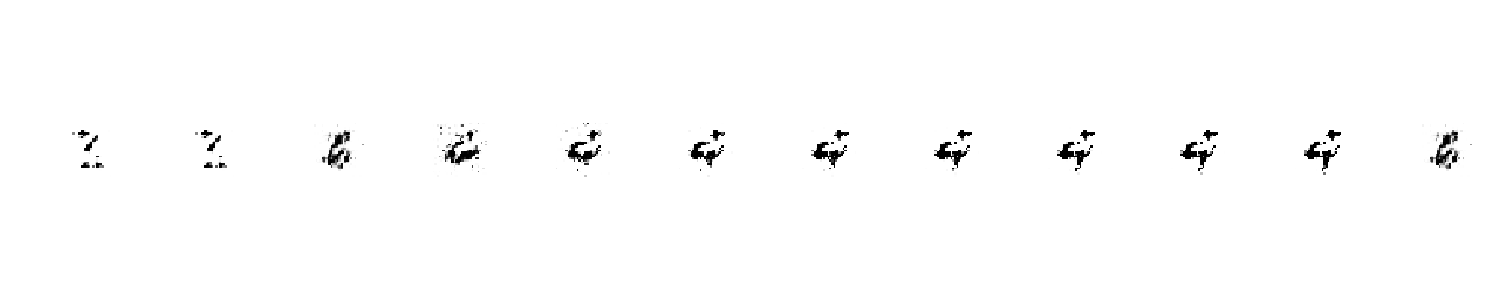
\includegraphics[width=15cm]{imgs/gan_12}
  \caption{\label{fig:gan_12} Two random latent vectors from the GAN space are sampled and the decoding of linearly interpolated latent vectors in between the two are decoded. We can see that the latent space is at least somewhat smooth.}
\end{figure}

\section{CNN VAE}
As an extension, we use a fully convolutional neural network as an autoencoder. The encoder is composed of leaky relus and batchnorms. The decoder is composed of several deconvolutions of either kernel 2, stride 2, and padding 0/1 depending on what worked to get the correct final dimensions. The network is trained in the exact same way as the original autoencoder of fully connected layers.\\
The same visualizations that were done for the original autoencoder are done for the convolutional one. By eye, the convolutional images look about identical to the original ones. The loss is shown in Figure \ref{fig:convloss}. The labeled scatter plot is shown in \ref{fig:convvaespace}. Figure \ref{fig:convgrid} shows an example linear interpolation. Figure \ref{fig:convlatent} shows the decoder evaluated on a grid of latent values.

\begin{figure}
  \centering
  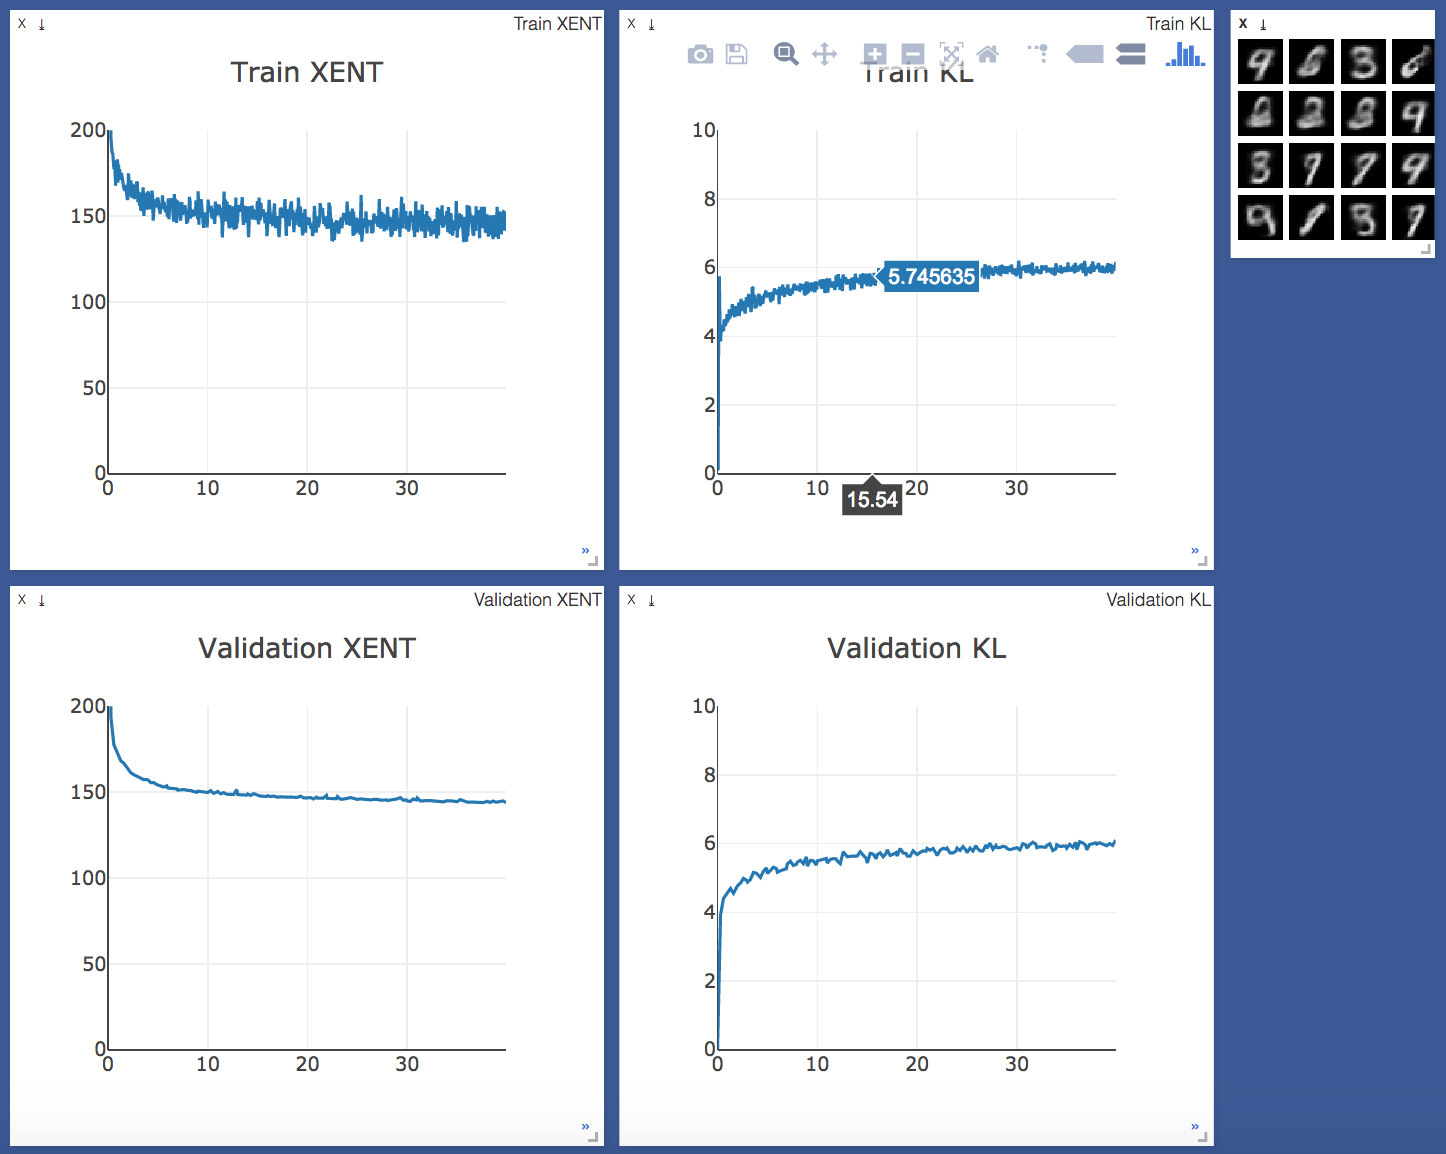
\includegraphics[width=9cm]{imgs/convtrain}
  \caption{\label{fig:convloss} Visualization of training and validation loss for the Convolutional VAE is handled by visdom. The x-axis is number of epochs through the training set in all cases. Example visualizations of the decoder's output in the top right are on random samples from $z$ which are sampled throughout training.}
\end{figure}

\begin{figure}
  \centering
  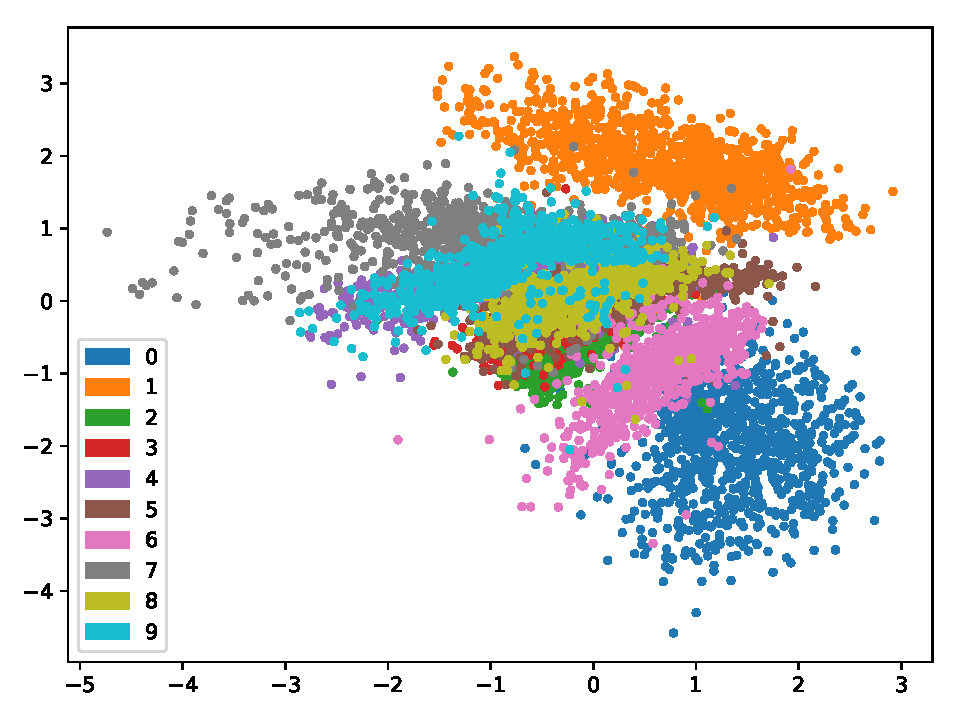
\includegraphics[width=9cm]{imgs/convvae_mus2}
  \caption{The Convolutional VAE model learns to separate the different digits without ever seeing a label. After training, on every test sample, we run the encoder and collect all the $\mu$ and ground truth labels. The $\mu$ are plotted and color coded by their ground truth label. The $\mu$ all together are roughly gaussian about the origin as enforced by the KL loss.}
  \label{fig:convvaespace}
\end{figure}

\begin{figure}
  \centering
  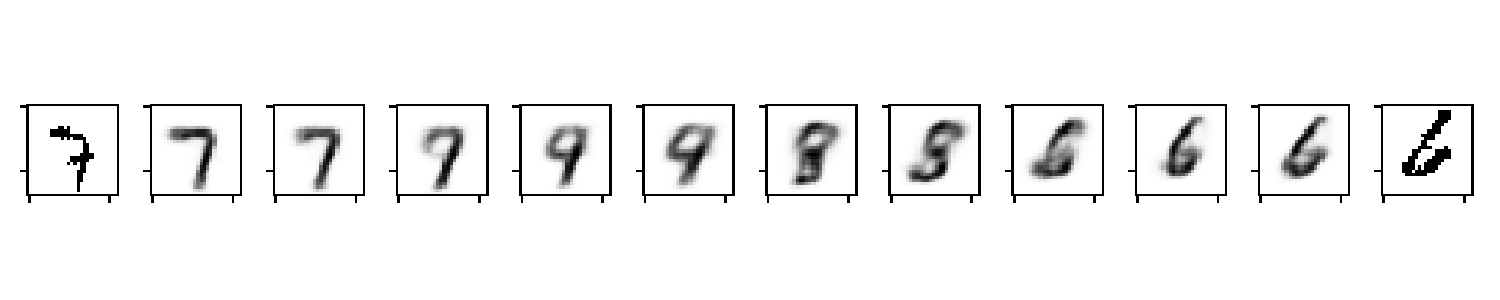
\includegraphics[width=15cm]{imgs/convinterp_vae1}
  \caption{\label{fig:convgrid} Two images from the test set are displayed on the far left and far right. We run the Convolutional VAE encoder on both images, then decode 10 interpolations between the latent vectors.}
\end{figure}

\begin{figure}
  \centering
  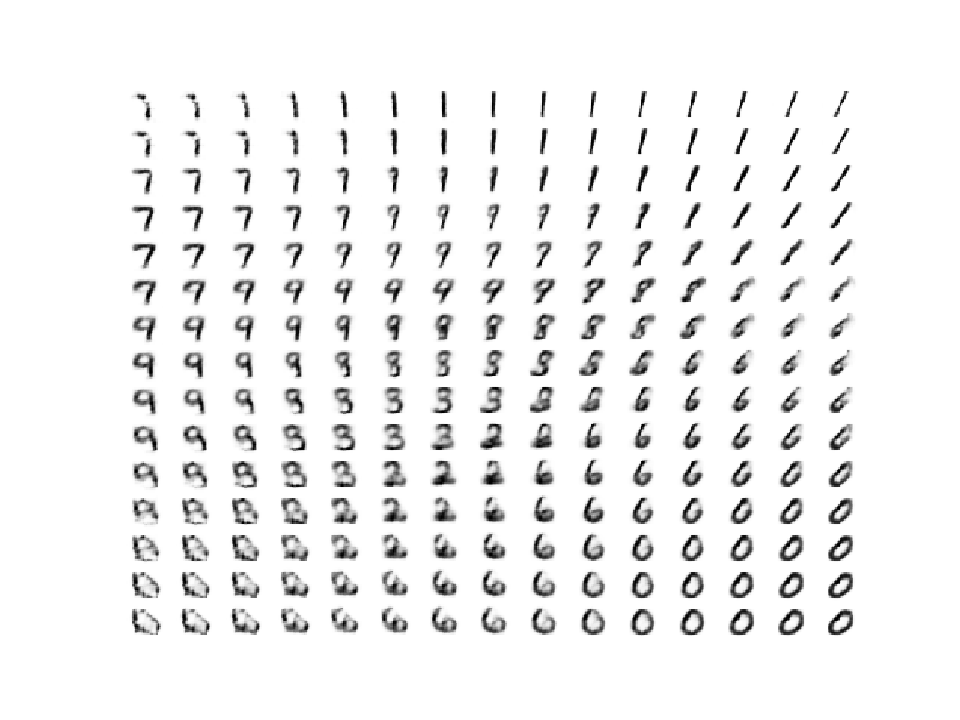
\includegraphics[width=15cm]{imgs/convgridvae}
  \caption{\label{fig:convlatent} 15 latent vectors from the Convolutional VAE latent space on a grid between -2 and 2 are decoded by the Convolutional VAE into images. This image looks similar to the standard VAE picture.}
\end{figure}



%\begin{itemize}
%\item Variational Autoencoder (VAE)
%\item Generative Adversarial Network (GAN)
%\end{itemize}
%
%%This note lays out our expectation for a homework submission in
%%\textit{CS287: Statistical Natural Language Processing}. While you do
%%not have to follow this template to the letter, we do expect that
%%write-ups have a very clear structure and cover all the elements
%%described in this note. With this in mind, the burden is on the
%%presenter to demonstrate why deviations from the standard are
%%necessary.
%%
%%All write-ups should include a short introduction. In this section you
%%should summarize the underlying problem in high-level language and
%%describe the extensions that you have decided to propose in your
%%implementation. When you describe these extensions you should
%%carefully cite the papers of interest. For instance, it will often be
%%useful to cite the work seen in class
%%\citep{murphy2012machine}. Alternatively, you can also cite papers
%%inline, for instance the work of \citet{berger1996maximum}.
%
%
%\section{Problem Description}
%Given a sentence in German of up to 20 words, we would like to predict a sentence in English with the same meaning.
%For all models, a sentence $\boldx_i$ is encoded as a sequence $x_1,...,x_n$ where each $x_j$ is a one-hot vector of length the vocabulary $\mcV$. The model outputs a categorical distribution over the vocabulary $\mcV$. Embeddings $\mcE_d$ map a one hot vector $x_j$ to a dense vector of size $d$. Each language gets its own word embedding.
%
%%In general, homeworks will be specified using informal
%%language. As part of the assignment, we expect you to write-out a
%%definition of the problem and your model in formal language. For this
%%class, we will use the following notation:
%%
%%\begin{itemize}
%%\item $\boldb, \boldm$;  bold letters for vectors.
%%\item $\boldB, \boldM$;  bold capital letters for matrices.
%%\item $\mcB, \mcM$;  script-case for sets.
%%\item $b_i, x_i$; lower case for scalars or indexing into vectors.
%%\end{itemize}
%%
%%
%%For instance in natural language processing, it is common to use
%%discrete sets like $\mcV$ for the vocabulary of the language, or $\mcT$ for a
%%tag set of the language.  We might also want one-hot vectors
%%representing words. These will be of the type
%%$\boldv \in \{0,1\}^{|\mcV|}$. In a note, it is crucial to define the
%%types of all variables that are introduced. The problem description is the
%%right place to do this.
%%
%%% NLP is also
%%% full of sequences. For instance sentences, $w_1, \ldots, w_N$, where
%%% here $N$ is a constant length and $w_i \in \mcV$ for all
%%% $i \in \{1, \ldots N\}$. If we pretend sentences are all the same
%%% length, we can have scoring function over sentences,
%%% $s : \mcV^N \mapsto \reals$.  One might be defined as:
%%
%%% \[ s(w_1, \ldots, w_N) = \sum_{i = 1}^N p(w_i | w_{i-2}, w_{i-1}), \]
%%
%%% \noindent where $p$ is the bigram probability, which we will cover later in the class.
%
%\section{Model and Algorithms}
%
%All models are trained on the \href{http://workshop2017.iwslt.org/}{IWLST}. For models requiring gradient descent, training loss and validation loss are recorded in real time with \href{https://github.com/facebookresearch/visdom}{visdom}. Reported PPL is on the validation set with teaching.
%
%\subsection{Evaluation}
%\begin{enumerate}
%\item All models assume a vocabulary of $10000$ and have a \ttfamily{predict} function which given a batch of sentence fragments outputs an array containing the probabilities for the next word for all batches.
%
%\item All models are tested with the same evaluation function. The function evaluates the model on batches of size 32 with the same metric used during training.
%\end{enumerate}
%
%
%
%%Here you specify the model itself. This section should formally
%%describe the model used to solve the task proposed in the previous
%%section. This section should try to avoid introducing new vocabulary
%%or notation, when possible use the notation from the previous section.
%%Feel free to use the notation from class, but try to make the note
%%understandable as a standalone piece of text.
%%
%%This section is also a great place to include other material that
%%describes the underlying structure and choices of your model, for
%%instance here are some example tables and algorithms from full
%%research papers:
%%
%%
%%
%%\begin{itemize}
%%\item diagrams of your model,
%%
%%  \begin{center}
%%    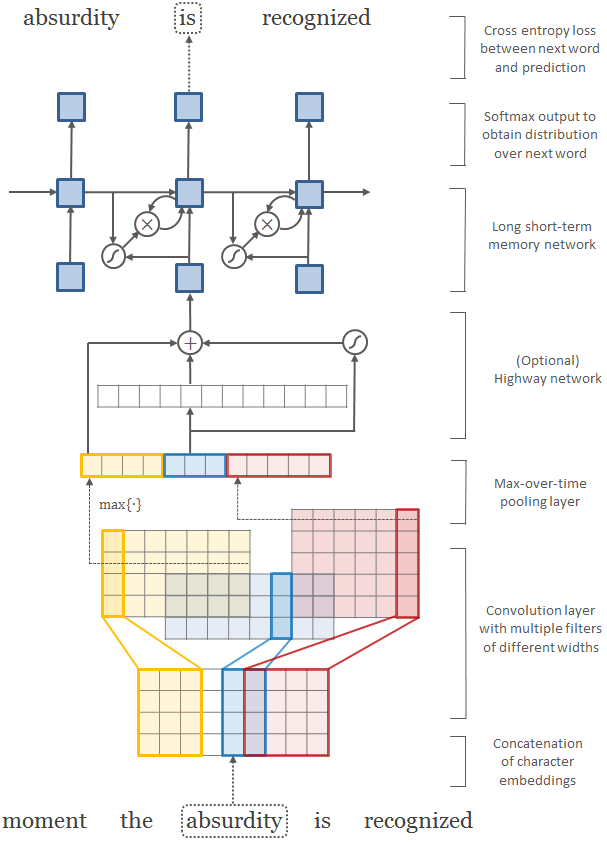
\includegraphics[width=0.4\textwidth]{network}
%%  \end{center}
%%\item feature tables,
%%
%%  \begin{center}
%%    \begin{tabular}{@{}lll@{}}
%%      \toprule
%%      &\multicolumn{2}{c}{Mention Features  } \\
%%      & Feature & Value Set\\
%%      \midrule
%%      & Mention Head & $\mcV$ \\
%%      & Mention First Word & $\mcV$ \\
%%      & Mention Last Word & $\mcV$ \\
%%      & Word Preceding Mention & $\mcV$ \\
%%      & Word Following Mention & $\mcV$\\
%%      & \# Words in Mention & $\{1, 2, \ldots \}$ \\
%%      & Mention Type & $\mathcal{T}$ \\
%%      \bottomrule
%%    \end{tabular}
%%  \end{center}
%%
%%\item pseudo-code,
%%
%%  \begin{algorithmic}[1]
%%    \Procedure{Linearize}{$x_1\ldots x_N$, $K$, $g$}
%%    \State{$B_0 \gets \langle (\langle \rangle, \{1, \ldots, N\}, 0, \boldh_0, \mathbf{0})  \rangle$}
%%    \For{$m = 0, \ldots, M-1$ }
%%    \For{$k = 1, \ldots, |B_m|$}
%%    \For{$i \in \mcR$}
%%    \State{$(y, \mcR, s, \boldh) \gets \mathrm{copy}(B_m^{(k)})$}
%%    \For{word $w$ in phrase $x_i$}
%%    \State{$y \gets y $ append $w$ }
%%    \State{$s \gets s + \log q(w, \boldh) $ }
%%    \State{$\boldh \gets \delta(w, \boldh)$}
%%    \EndFor{}
%%    \State{$B_{m+|w_i|} \gets B_{m+|w_i|} + (y, \mcR - i, s,   \boldh)$}
%%    \State{keep top-$K$ of $B_{m+|w_i|}$ by $f(x, y) + g(\mcR)$}
%%    \EndFor{}
%%    \EndFor{}
%%    \EndFor{}
%%    \State{\Return{$B_{M}^{(k)}$}}
%%    \EndProcedure{}
%%  \end{algorithmic}
%%
%%\end{itemize}
%
%
%\section{Experiments}
%Both models are trained with Adam Optimizer .001 learning rate, weight\_decay .0001 for 10-20 epochs 
%\begin{subsection}{No Attention}
%To encode, we reverse the input sentence, then embed the sentence in a space of dimension $200$. An LSTM of one direction, 4 layers deep, with initialized state and hidden layers to 0, reads through the sentence and we store the final hidden layers and state, as well the history of the hidden layer throughout the sentence.\\
%To decode, we embed the ground truth $trg$, run a LSTM with initial hidden state and state given by the output of the encoder. The hidden state $h_t$ of the decoder LSTM at any $t$ is projected to $V$ by a linear layer $D \rightarrow V_{en}$. The graph during training is shown in Figure \ref{fig:noatt}.\\
%With beam search of $B=5$ the top scoring sentences of the first three sentences are
%\centerline{PPL: 8.02}
%\centerline{{\bf src:} Als ich in meinen 20ern war , hatte ich meine erste Psychotherapie-Patientin .}
%\centerline{{\bf model:} And when I was in my <unk> , I 've got my first <unk> . "}
%\centerline{{\bf Google:} When I was in my 20s, I had my first psychotherapy patient.}
%\centerline{}
%\centerline{{\bf src:} Ich war Doktorandin und studierte Klinische Psychologie in Berkeley .}
%\centerline{{\bf model:} So , I was <unk> and <unk> <unk> <unk> in <unk> . <unk> .}
%\centerline{{\bf Google:} I was a PhD student and studied Clinical Psychology in Berkeley.}
%\centerline{}
%\centerline{{\bf src:} Sie war eine 26-jährige Frau namens Alex .}
%\centerline{{\bf model:} And it was a <unk> man called <unk> <unk> .}
%\centerline{{\bf Google:} She was a 26-year-old woman named Alex.}
%
% \begin{figure}
%  \centering
%  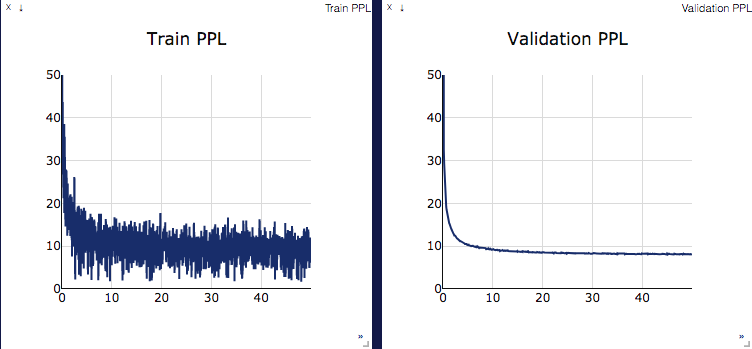
\includegraphics[width=6cm]{imgs/noatt}
%  \caption{\label{fig:noatt} The network just barely reaches a PPL of 8.}
%\end{figure}
%
%%Word counts for positive and negative labels are all initialized to a global initial count of $\alpha$. Figure \ref{fig:clusters} shows that performance of the algorithm on the validation set is robust to changes in $\alpha$. With $\alpha=.5$, performance on the test set using binarized and count word vectors are analyzed in Table \ref{tab:nb}.\\
%%The weight vector determined by Naive Bayes can be interpreted as the sentiment associated with particular words. The most positive and most negative words and their weights for binarized bag of words are shown in Table \ref{tab:nbwords}.
%%
%%
%%
%%
%%
%%\begin{table}[h]
%%\centering
%%\begin{tabular}{llrrr}
%% \toprule
%% Model &  & Acc. & Bce. & Roc.\\
%% \midrule
%% \textsc{Binarized} & & 0.791 & 0.679 & 0.867\\
%% \textsc{Counts} & & 0.793  & 0.686 & 0.867\\
%% \bottomrule
%%\end{tabular}
%%\caption{\label{tab:nb} Binarizing or counting words does not significantly affect the performance of the model on the test set.}
%%\end{table}
%%
%%
%%
%%\begin{table}[h]
%%\centering
%%\begin{tabular}{cccccccccc}
%% \midrule
%% stupid & unfunny& pointless  & poorly & suffers & Feels & tiresome & car \\
%%   5.39452 & 5.1085& 5.03998 &4.96641&4.96641 & 4.88701 & 4.88701 & 4.88701 \\
%% \bottomrule
%% \bottomrule
%% powerful  & solid& perfectly & inventive & refreshing & riveting & wonderfully & universal \\
%%  -5.79766 & -5.7109 & -4.99019 & -4.85754 & -4.78398 & -4.70458 & -4.61832 & -4.61832 \\
%% \bottomrule
%%\end{tabular}
%%\caption{\label{tab:nbwords} Words with the highest and lowest weights in the naive bayes weight vector agree with intuition for being negative and positive words respectively.}
%%\end{table}
%
%\end{subsection}
%
%
%
%
%\begin{subsection}{Attention}
%
%The encoder is no different from that of the non-attention model.\\
%For the decoder, the embedding of the source sentence is first padded with zeros to be a length of 20. Next, the most recent hidden state is concatenated to the most recent word vector and fed to a linear layer $2D \rightarrow 20$. The softmax of this vector gives the ``attention" to the at most 20 words in the source sentence. The input to the decoder is a linear combination of the encoding with coefficients given by the ``attention" vector concatenated with the input word vector. As in the no-attention model, a linear layer $D \rightarrow V_{en}$ gives the output distribution over the vocabulary. I report the score for $D=300$.\\
%\centerline{PPL: 7.97}
%The training graph is shown in Figure \ref{fig:att}. An example translation is below.
%
% \begin{figure}
%  \centering
%  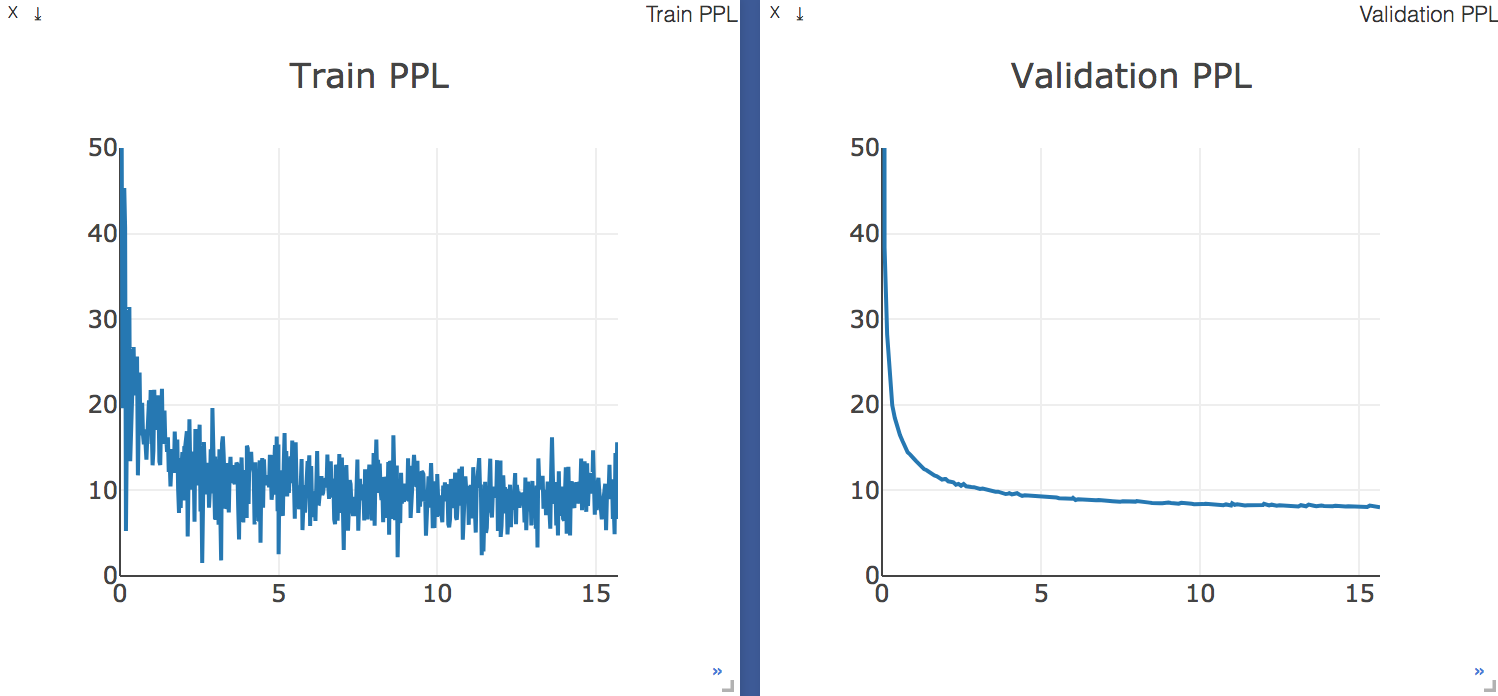
\includegraphics[width=6cm]{imgs/att}
%  \caption{\label{fig:att} The network performs almost identically to the non attention model which means that the attention component of the decoder was just noise.}
%\end{figure}
%
%\centerline{{\bf src:} Als ich in meinen 20ern war , hatte ich meine erste Psychotherapie-Patientin .}
%\centerline{{\bf model:} And when I was <unk> <unk> , I was my first <unk> . I said .}
%\centerline{{\bf Google:} When I was in my 20s, I had my first psychotherapy patient.}
%\centerline{}
%\centerline{{\bf src:} Ich war Doktorandin und studierte Klinische Psychologie in Berkeley .}
%\centerline{{\bf model:} And it was <unk> <unk> , and I was <unk> in <unk> <unk> .}
%\centerline{{\bf Google:} I was a PhD student and studied Clinical Psychology in Berkeley.}
%\centerline{}
%\centerline{{\bf src:} Sie war eine 26-jährige Frau namens Alex .}
%\centerline{{\bf model:} She was a woman called <unk> <unk> . He said .}
%\centerline{{\bf Google:} She was a 26-year-old woman named Alex.}
%
% \begin{figure}
%  \centering
%  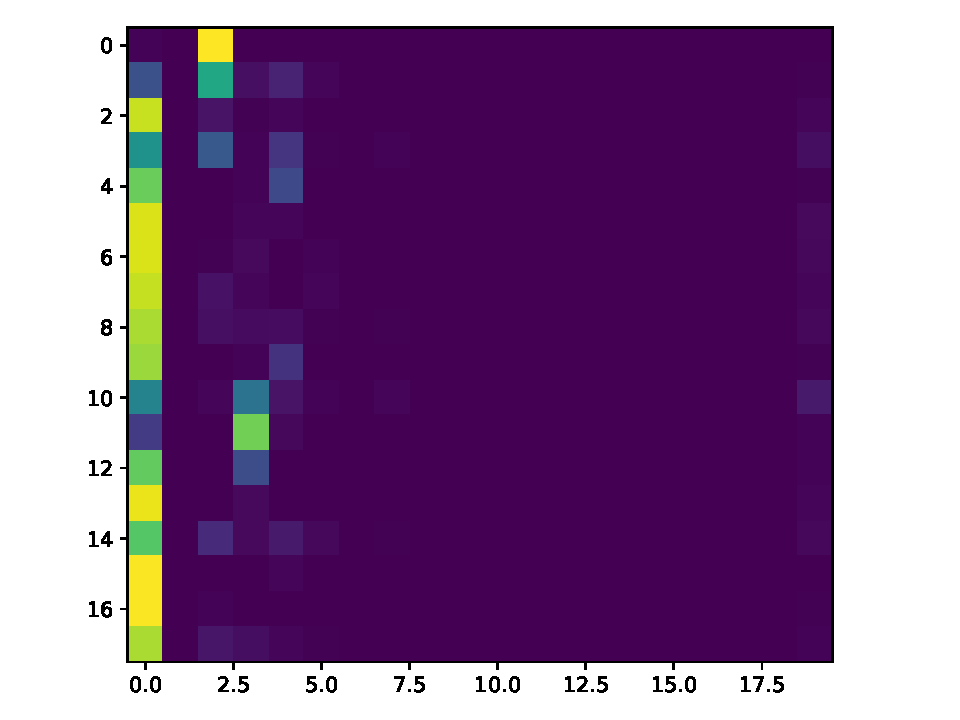
\includegraphics[width=6cm]{imgs/att_fig}
%  \caption{\label{fig:att_fig} The attention does not look good. The horizontal axis is the maximum sentence length of 20, the vertical axis corresponds to each word generated in the output sequence. The sum of each row is 1.}
%\end{figure}
%
%\end{subsection}
%
%
%
%
%
%
%%Finally we end with the experimental section. Each assignment will make clear the main experiments and baselines that you should run. For these experiments you should present a main results table. Here we give a sample Table~\ref{tab:results}. In addition to these results you should describe in words what the table shows and the relative performance of the models.
%%
%%Besides the main results we will also ask you to present other results
%%comparing particular aspects of the models. For instance, for word
%%embedding experiments, we may ask you to show a chart of the projected
%%word vectors. This experiment will lead to something like
%%Figure~\ref{fig:clusters}. This should also be described within the
%%body of the text itself.
%%
%%
%%\begin{table}[h]
%%\centering
%%\begin{tabular}{llr}
%% \toprule
%% Model &  & Acc. \\
%% \midrule
%% \textsc{Baseline 1} & & 0.45\\
%% \textsc{Baseline 2} & & 2.59 \\
%% \textsc{Model 1} & & 10.59  \\
%% \textsc{Model 2} & &13.42 \\
%% \textsc{Model 3} & & 7.49\\
%% \bottomrule
%%\end{tabular}
%%\caption{\label{tab:results} Table with the main results.}
%%\end{table}
%%
%%
%%\begin{figure}
%%  \centering
%%  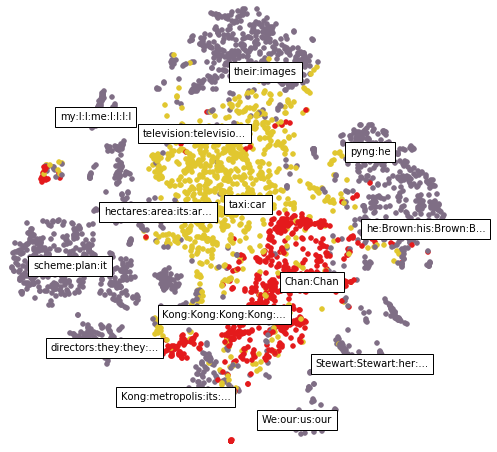
\includegraphics[width=6cm]{cluster_viz}
%%  \caption{\label{fig:clusters} Sample qualitative chart.}
%%\end{figure}
%
%
%%\section{Conclusion}


\end{document}
